\section{Methodology}

For the realization of our concept, the following three objectives have to be accomplished:

\begin{enumerate}
    \item Obtaining of a sufficiently large data set with different expressions about the topic of AI.
    \item Raw data transformation into a data set that to the target schema illustrated in Table~\ref{data-schema}
    \item Creation of a visualization from which society's perceptions on different topics of AI can be extracted.
\end{enumerate}%
%
%
\begin{figure}[t]
    \centering
    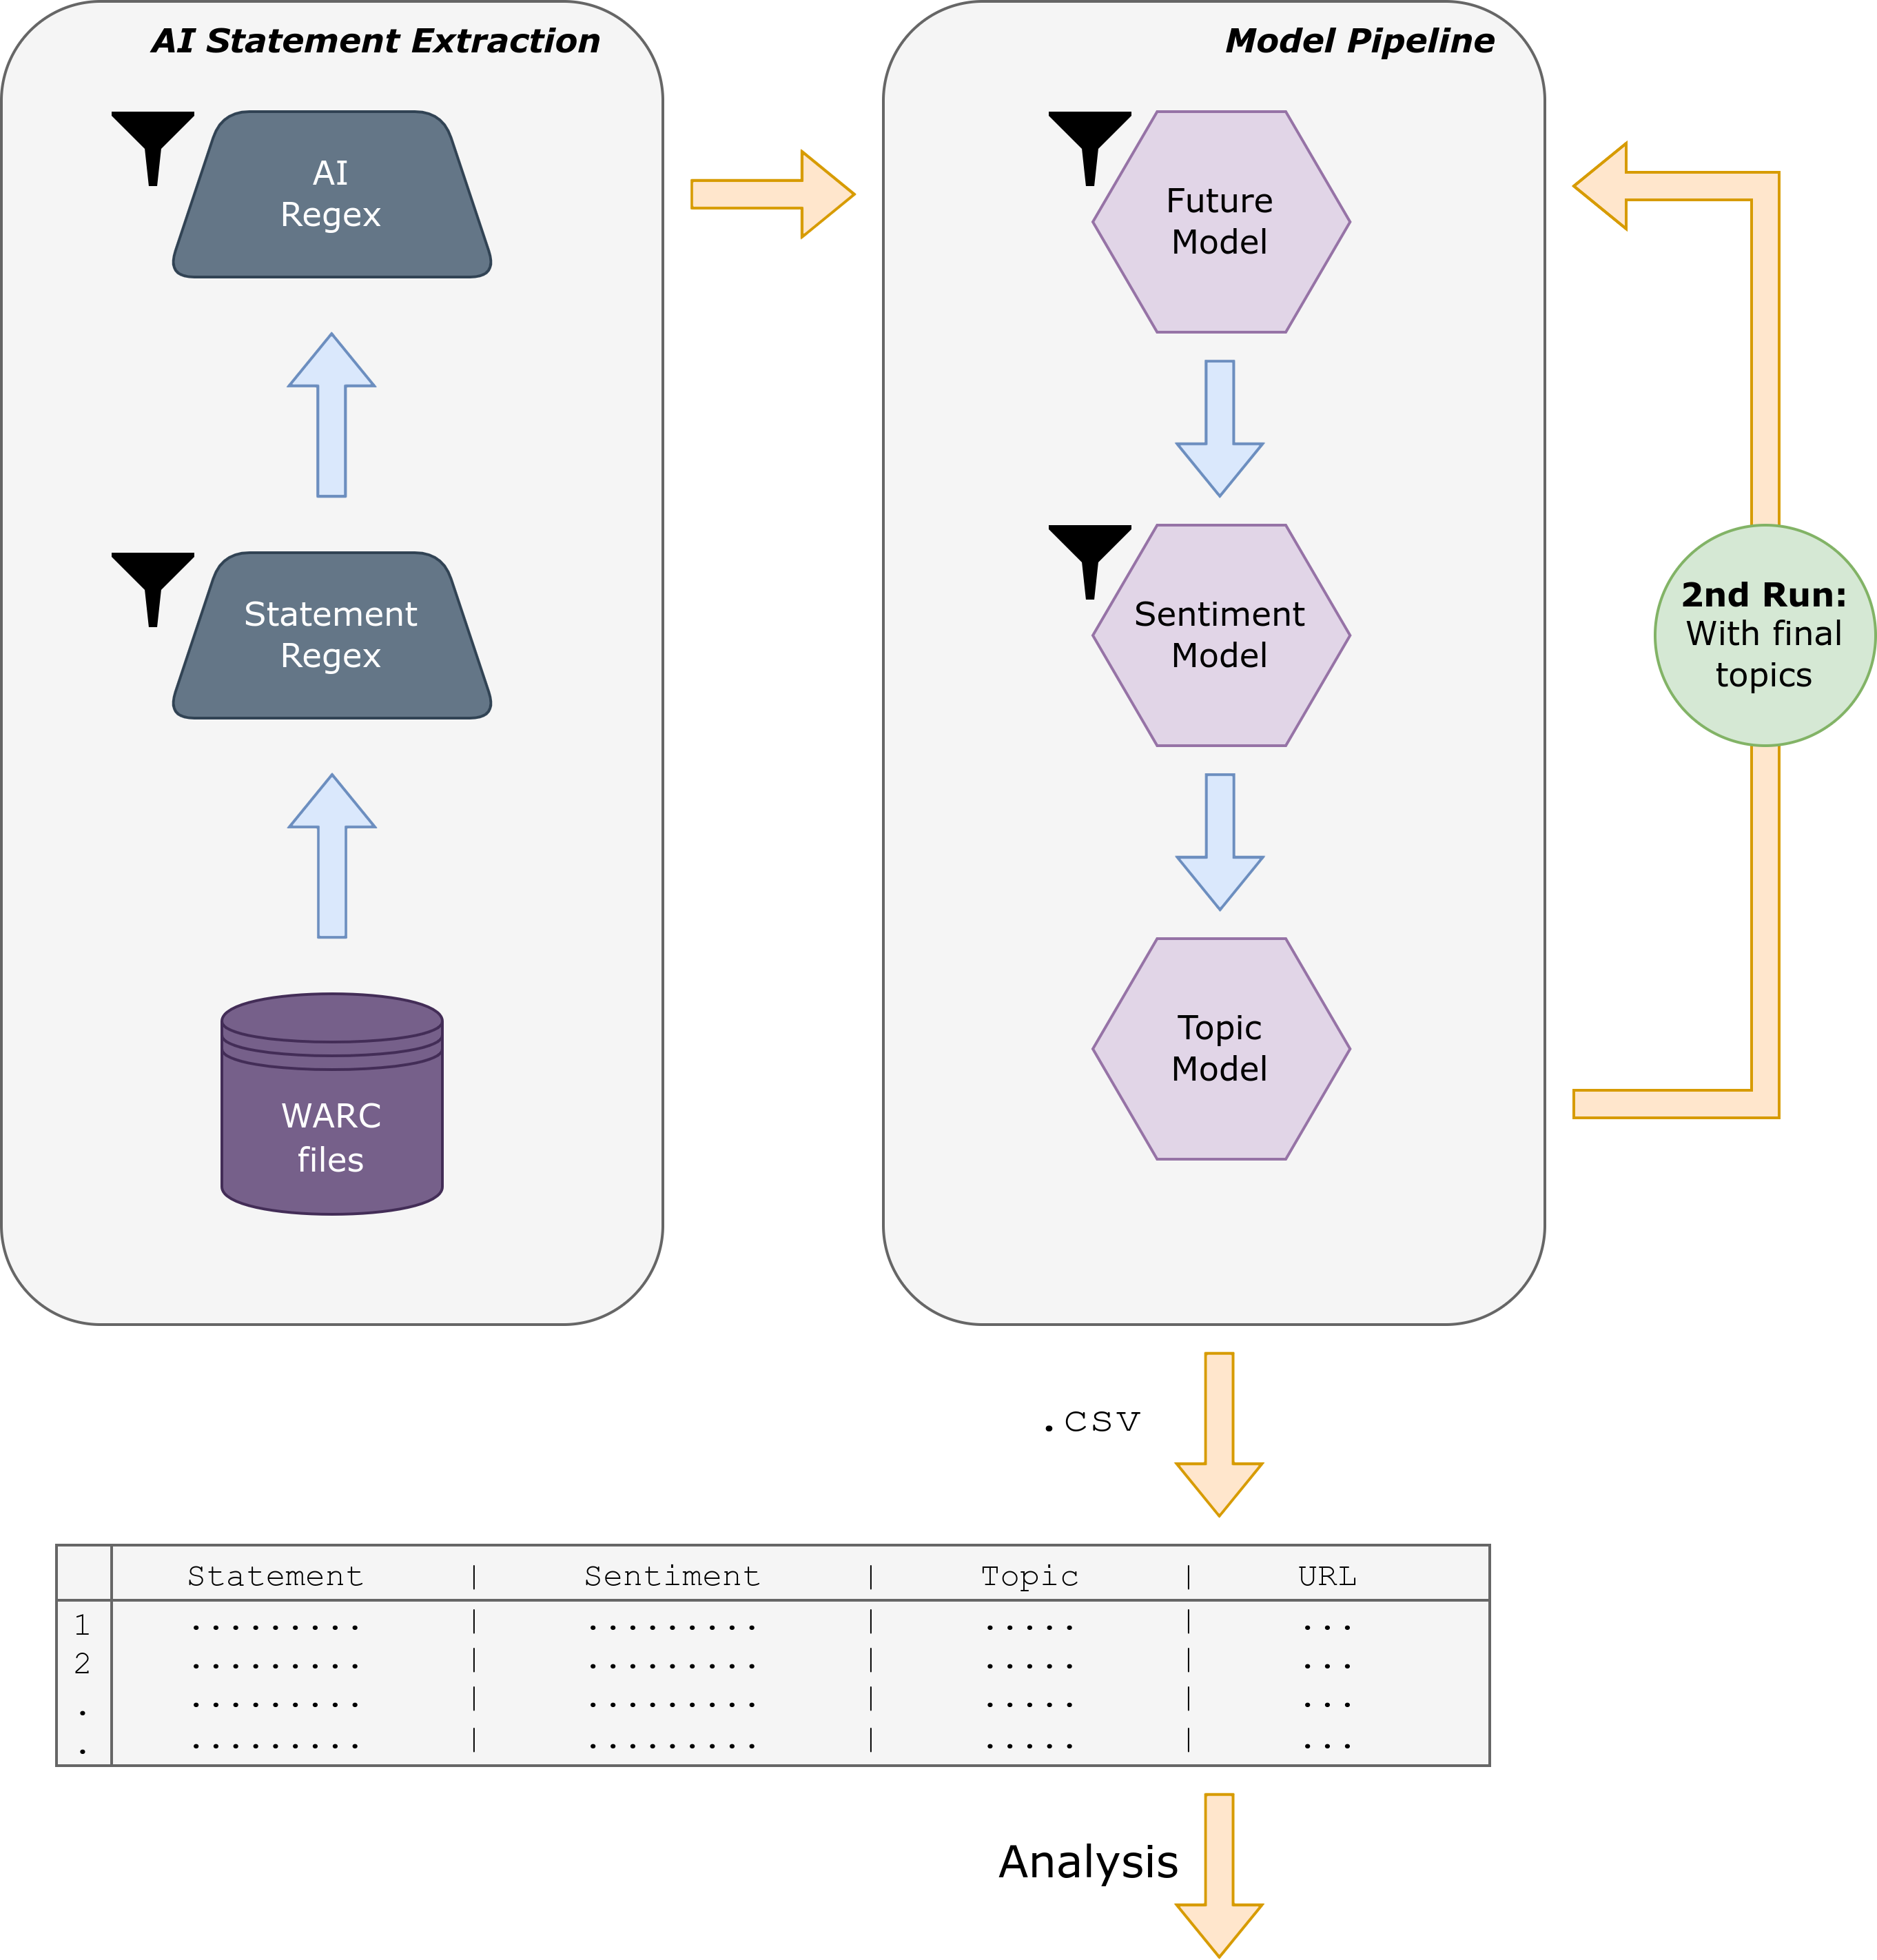
\includegraphics[width=\linewidth]{overview}
    \caption{
        The statement extraction, filter and final topic assignment process.
        AI statements are extracted from website HTMLs located inside WARC files (left part).
        The extraction process involves the application of two regexes (statement regex and AI regex).
        Statements then enter the model pipeline (left side), where they are further filtered through the future model and the sentiment model.
        The model pipeline runs two times in total. The first time the topic model assigns dummy topics.
        After the topic selection process (green circle), where we fine-tune the topic model, the model pipeline runs a second time.
        Now the topic model assigns the final topics to the statements.
        The output is a \texttt{.csv} file with the schema \texttt{statement|sentiment|topic|url}.
    }
    \label{fig:overview}
\end{figure}
\underline{1. WARC Data Extraction:}
\\
Initially, we outline the raw data acquiring containing AI expressions.
Since the web archive provided by the Webis group with the corresponding WARC-DL data extraction pipeline \citep{Deckers2022} is at our disposal, we utilize those.
The data set consists of long texts.
For that reason, the text must be split into separate sentences.
Then, sentences about AI can be extracted for later processing by applying Regex.
\\
\\
%
\underline{2. Data Transformation:}
\\
For later analysis, the data must be converted to required target schema, illustrated in Table~\ref{data-schema}. Therefore we employ the model pipeline, which generates the final data set with the attributes future statement, sentiment, topic and url. Within this model pipeline three models are applied sequentially:
\begin{itemize}
    \item Future statements model:\\
    This model is able to distinguish between statements about the future and all other types of terms.
On the basis of its classifications, statements about the future are extracted.
    \item Sentiment model:\\
A sentiment is assigned to every future statement by this model
    \item Topic model: \\
    Before our selected topic model enables the assignment of reasonable topics, those must be provided as label candidates to this topic model.
Accordingly, the Model Pipeline runs twice. In the first execution the chosen model runs with dummy topics. Based on the output the topic selection is conducted.
For each subsequent run, the model pipeline is considered complete.
\end{itemize}

The URLs of the pages are also included in the data schema for a later discussion. This pipeline generates the final data set with the attributes future statement, sentiment, topic and URL. The resulting data set can then be used for analysis and interpretation.
\\
\\
\underline{3. Analysis:}
\\
For the analysis we start with a graphical visualization.
Therefore, we decided to group all statements according to their topics.
This way for every topic a sentiment analysis can be conducted separately.
\\
\\
In the following sections, each step of the implementation is discussed in detail.


\begin{table}[t]
    \centering
    \resizebox{\columnwidth}{!}{%
    \begin{tabular}{llll}
        \toprule
        \textbf{statement} & \textbf{sentiment} & \textbf{topic} & \textbf{url} \\
        \midrule
        AI can be a risk for many workers. & NEG & finances & ... \\
        AI will definitely revolutionize games! & POS & gaming & ... \\
        ... & ... & ... & ... \\
        \bottomrule
    \end{tabular}
    }
\caption{\label{data-schema}
Data schema for visualization and analysis
}
\end{table}


\subsection{WARC Data Extraction}
The Webis Group\footnote{\url{https://webis.de}} had provided us with access to 37908 WARC files, with a total amount of \highlight{XXXXXXTB} of website data, and a high-performance computer cluster where we were able to schedule jobs.
Additionally, we decided to utilize the WARC-DL pipeline \citep{Deckers2022}, a Python software pipeline tightly coupled with the WARC endpoint, and using the FastWARC\footnote{\url{https://resiliparse.chatnoir.eu/en/stable/man/fastwarc.html}} library under the hood to iterate over WARC records.
It enabled us to extract text automatically from the WARC records using several customizable filters.
We made some slight modifications to the source code, in order to make it fit our needs better.
\\
Since we were going to analyze AI statements, we did not need all of the text provided by a website html, but grammatically correct statements of the English language.
It is not possible to extract all statements with an accuracy of 100\% using regex only, so we narrowed it down to passages which started with a capital letter and ended with a period or exclamation mark.
We built a regex pattern which extracted a list of all valid statements from a html source.
\\
Furthermore, we were only interested in statements about AI, so we compiled a list of AI keywords beforehand and applied a second regex on the extracted statements.
We compiled a blacklist which contained keywords for filtering out hostnames related to pornographic websites, and a whitelist to only accept top level domains which were most common, and where the websites most likely contained English text.
This was necessary, since initial runs of the WARC-DL pipeline extracted lots of unusable content (including content in languages other than English).
\\
We ran into some problems with the cluster and WARC-DL pipeline, so we could not extract all statements in one job run.
Jobs would suddenly stop extraction because of connection errors or out-of-memory errors, and halt with an Exception.
We separated hostnames in four groups depending on the initial hostname character: \texttt{a-h}, \texttt{i-p}, \texttt{q-x} and \texttt{yz0-9}.
This way we could pin down the problematic websites more precisely.
In the end we managed to work through all WARC files in group \texttt{i-p} and \texttt{yz0-9}, and most of the WARC files in groups \texttt{a-h} and \texttt{q-x}.
The final yield of the WARC data extraction stage was a total amount of 222246 AI statements.
In the next steps, starting with the model pipeline, our objective was to further refine this initial data set.

\subsection{Model Pipeline}
The model pipeline follows the WARC data extraction step and is designed to prepare our final data set, which consists of the future statements and their associated sentiment and topic labels.
The processing within the model pipeline is performed on batches of 30 records each from the WARC-DL output.
\\
First the future model filters out future statements from the corresponding batch.
Subsequently, the chosen sentiment model assigns a sentiment to each future statement.
In this step some future terms can be sorted out.
This concerns the statements to which a sentiment is classified with a probability of less than 70\%.
The remaining future statements receive a topic.
Finally those are persisted in a csv file.
\\
In the following sections \ref{future-model} - \ref{topic-model} we will go into detail about each individual model.
In this context, we describe how the future model was trained and justify our decision for the sentiment and the topic model selection.
Furthermore we outline the choice of our topics and explain, why only those statements are kept which a sentiment with a probability above 70\% can be attributed.

\subsection{Future Model}
\label{future-model}
Since this paper focuses on analyzing statements about the future, a system for distinguishing between future statements and other expressions is required.
In this context, we decided to finetune the DistilBERT \citep{Sanh2019DistilBERTAD} base model that accomplishes this task.
Therefore, in this subsection, the collection of appropriate training data and the subsequent finetuning of the corresponding model is thematized.

\subsubsection{Training Data Set}
\label{training}
In order to provide a suitable data set to establish the future model, we adopted multiple approaches.
At this point, our goal was to compose the data in such a way that we would have a balanced data set with two classes.
The first class should contain future statements and the second all other types of terms.
While two of our group members manually annotated 500 observations each, the other two used an automated mechanism with subsequent verification of the collected data.
\\
One of the automatized approaches involves a web crawler developed on the basis of the python library Beautiful Soup \citep{Richardson2022}.
The text on a page is divided into sentences.
Subsequently every sentence is examined for occurrence of certain terms, as \emph{going to}, \emph{will}, \emph{won't} or \emph{'ll}.
\\
The second automated approach is the sentence extraction tool, which works in several aspects, similar to the web crawler.
At the beginning, it searches the given directory for text files.
If those exist the text is split into sentences and observed for specific expressions, as described above.
\\
To find the phrases that are not future statements, both the web crawler and the sentence extraction tool look only at the corresponding records that do not contain the previously considered expressions.
A careful manual review of all terms gathered by the automated systems was subsequently performed to remove the incorrect records.
\\
Finally, we constructed a data set with 1250 future statements and 1250 other phrases that did not contain future statements.

\subsubsection{Training}
As previously described we used the DistilBERT base model and finetuned it with the data set specified in \ref{training}.
We split the data set of 2500 records into a training and a test set, where the test set contains 20\% of the records.
From the training set we split further 20\% for validation data.
\\
After only two epochs the training ended with an accuracy over 96\% as displayed in (Table~\ref{future-model-train}).
\\
Subsequently we tested the model on our test set containing 500 records never seen by the model and achieved an accuracy of 93.8\%, as seen in the confusion matrix in (Table~\ref{cm}).


\subsection{Sentiment Model}
In order to assign sentiments to future statements for later analysis, we decided to select a ready-trained model.
The chosen sentiment model is the SentimentAnalyzer of the open-source library pysentimiento \citep{perez2021pysentimiento}, which was further trained on about 40k tweets.
It uses the BERTweet \citep{bertweet} as a base model, pre-trained on english tweets.

\subsubsection{Evaluation}
To evaluate the SentimentAnalyzer, we annotated 604 future statements, which were previously used for training the future model, as negative, positive or neutral and received an accuracy of about 65\%.
\\
We then analyzed all misclassified statements.
We noticed that some of the statements could not be assigned impartially to one of the three categories.
An Example is \emph{``AI will reinvent how we think about education''}.
In the case of the sentence, we disagreed on whether we should value the sentence as neutral or positive and decided to use the neutral label.
Subsequently, this statement was given a positive rating by the model.
On closer examination of the statements that were labeled differently by us and by the model, we found over 90\% of the labels given by the model to be valid, if these annotations were assigned with probability over 70\%.
For this reason, we decided to keep only statements about the future if the sentiment model assigned an annotation with a confidence above 70\%.

\subsection{Topic Model}
\label{topic-model}
\begin{figure}[t]
    \centering
    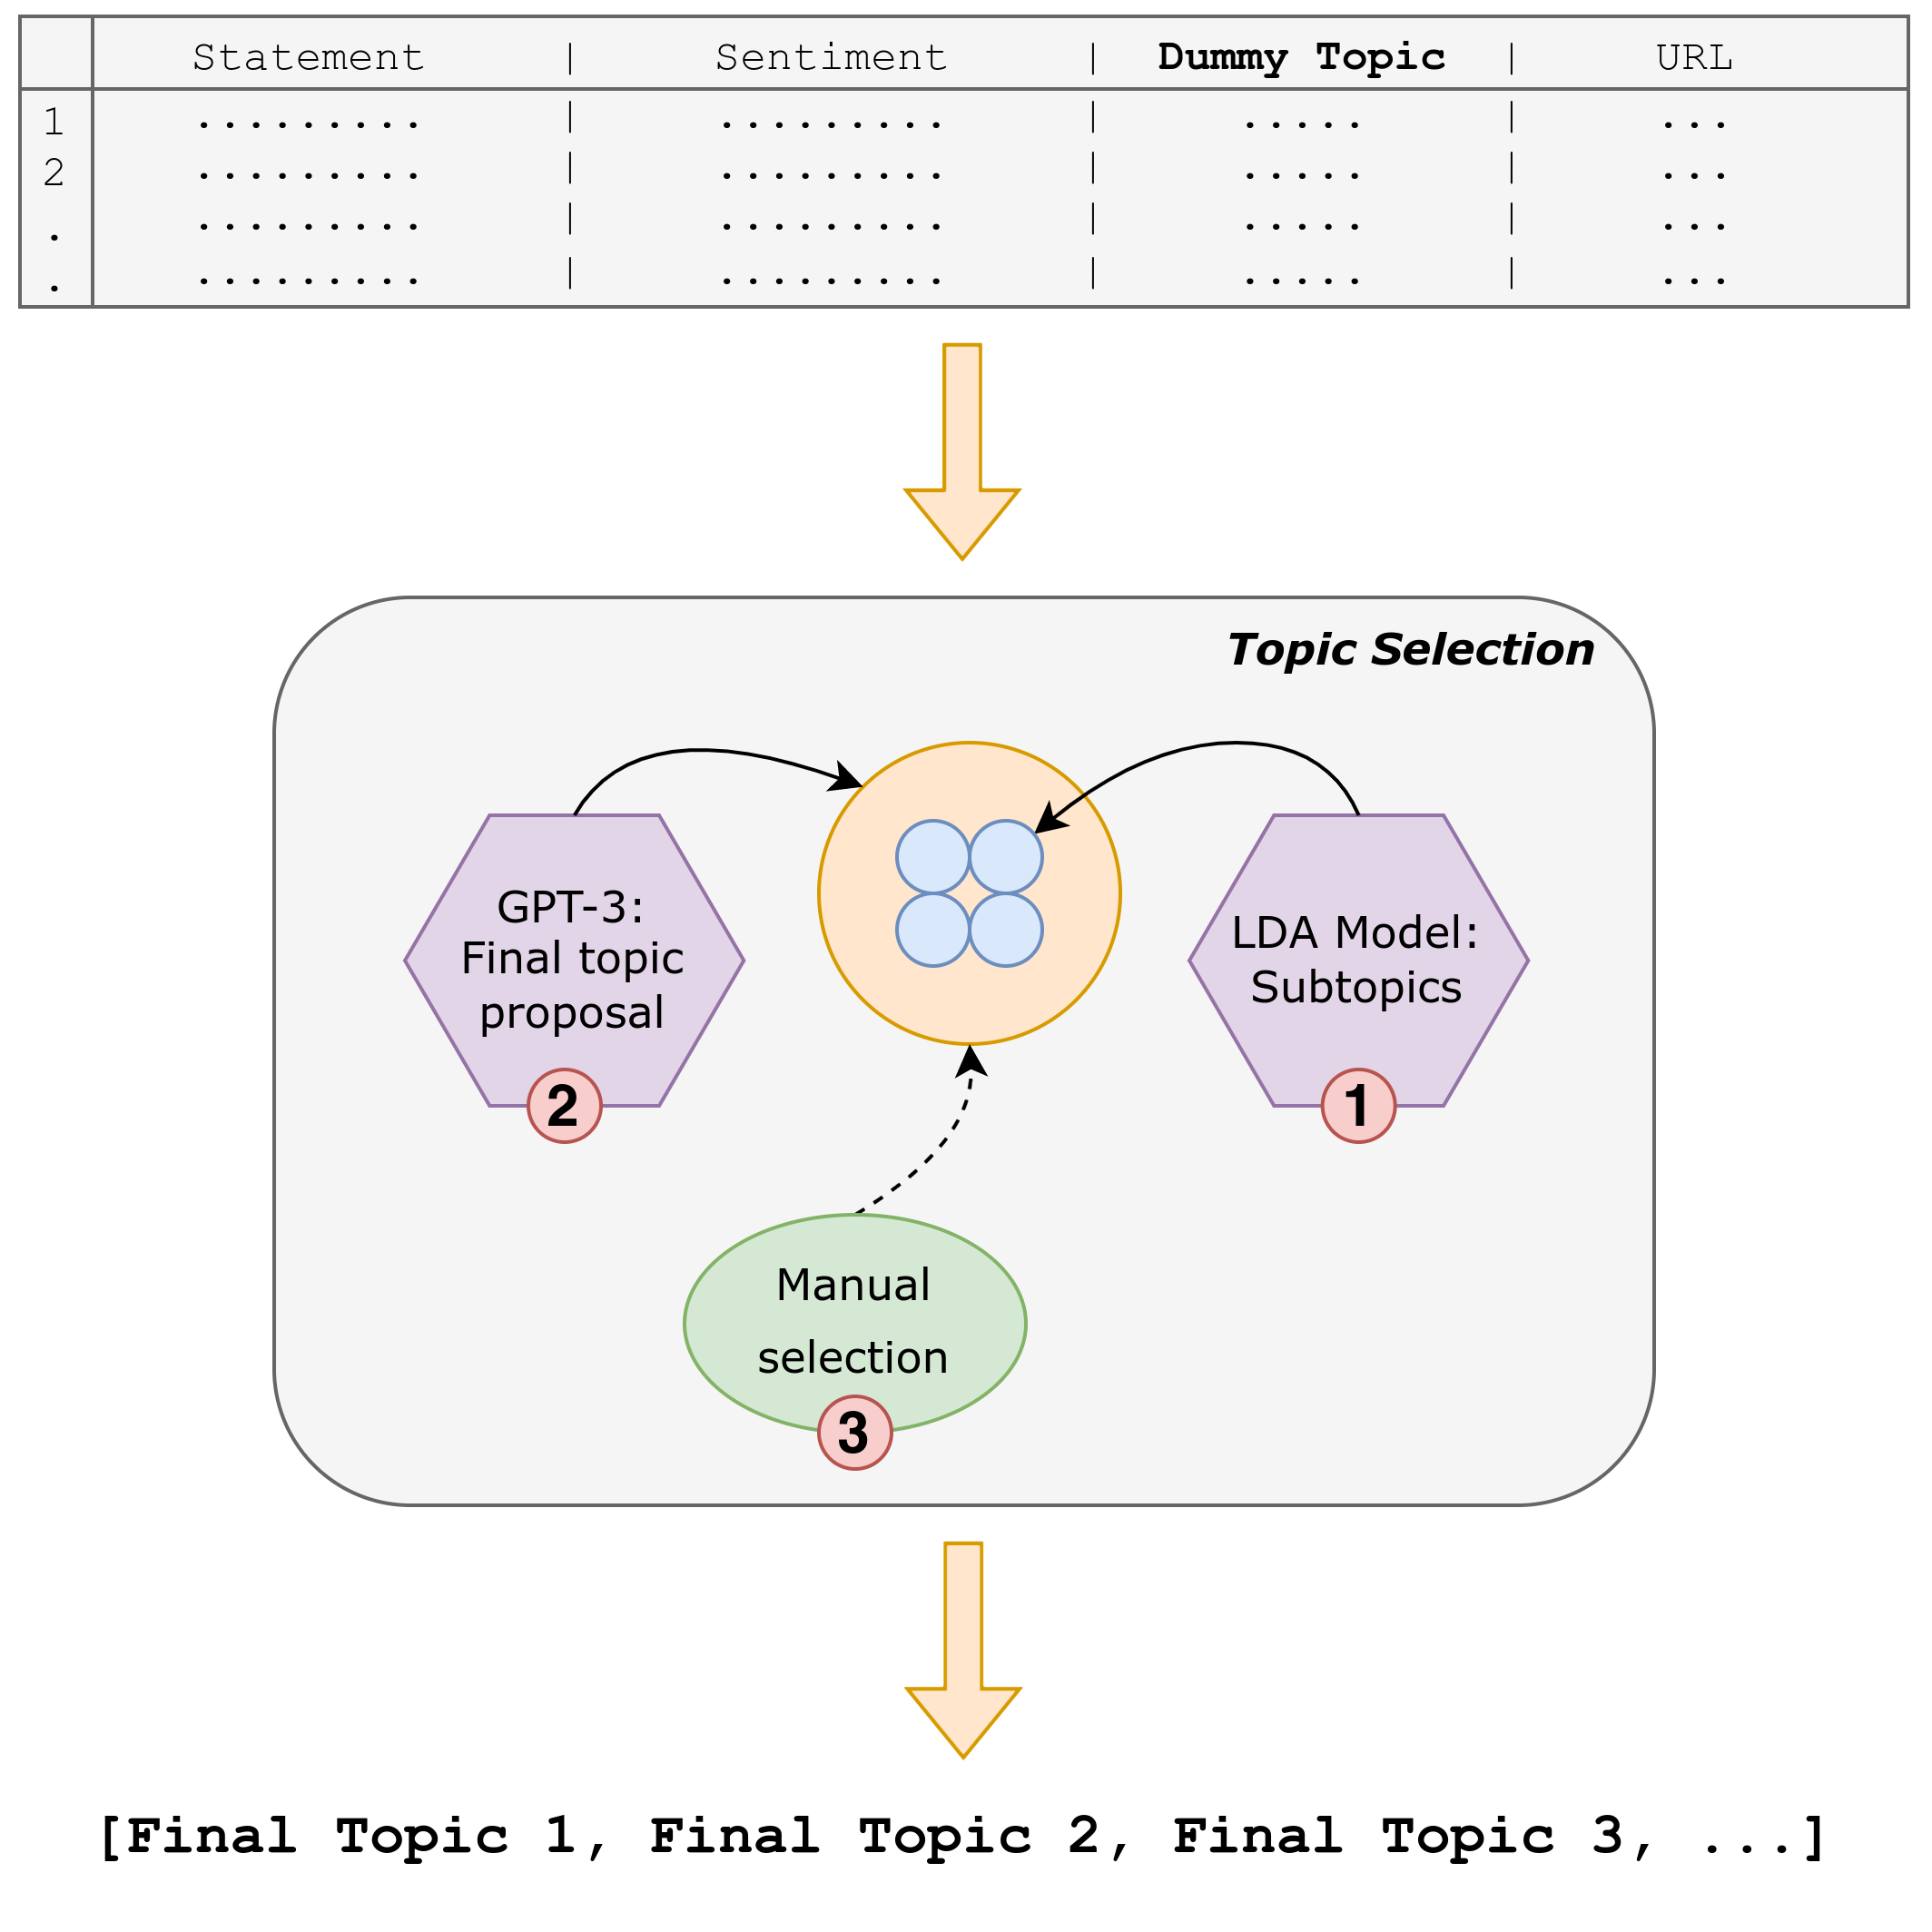
\includegraphics[width=\linewidth]{topic_selection}
    \caption{
        The three steps of topic selection.
        First, the LDA Model generates a set of subtopics for a topic cluster.
        In this example, there are four subtopics (small blue circles).
        Then, GPT-3 proposes a possible general topic for the subtopic set (large yellow circle).
        Lastly, we either pick this final topic as proposed, or replace it with a more suitable one from the same category, e.g. \texttt{level} would become \texttt{gaming}.
    }
    \label{fig:topic_selection}
\end{figure}
For assigning topics to the future statements we employ the bart-large-mnli model from Facebook, which was pretrained on the MultiNli \citep{N18-1101} data set, which consists of 433000 pairs of sentences annotated with textual supplementary information. The bart-large-mnli is a natural language processing model based on the technique of \citet{yin2019benchmarking} utilizing pre-trained NLI models as ready-to-use zero-shot sequence classifiers.
The approach involves specifying the sequence for classification as an NLI prerequisite and then constructing a hypothesis of every possible label candidate.
Afterwards probabilities of agreement and contradictions are transformed into annotation probabilities.
Before we are able to use the bart-large-mnli it is necessary to define the topics, which can be assigned to every statement by this model.
For instance, to verify if a sentence is a political or a technological statement, we can provide the model with the label candidats politics and technology. Then the model will apply one of the labels to the sentence.
In the following section our topic selection approach is described in detail.

\subsubsection{Topic Discovery with LDA}
For analyzing the overarching topics within our future statements, we used Latent Dirichlet Allocation (LDA). LDA is a subtype of the Dirichlet Process Mixture Models (DPMMs), a set of non-parametric, “fully-Bayesian” unsupervised clustering models which are commonly used for topic cluster analysis. DPMMs use a stochastic process to generalize the Dirichlet distribution (the conjugate prior for a categorical or multinomial distribution) for infinitely many categories \citep{li2019tutorial}.
Applied to NLP, a Latent Dirichlet Allocation model clusters observations into unobserved groups of related data. It has the advantage of following a generative process that is immune to overfitting with increasing size of the data corpus and can be scaled to a data cluster in machine learning \citep{pritchard2000inference}
\\
\\
We prepared our data set for LDA by removing punctuation, words with less than three letters and stopwords. The cleaned data was then converted into lowercase and fed into a tokenizer. From there on, we created bigrams (sets of two words) from the tokens and employed a Word2Vec model to select only the most occuring ones.
Finally, bigrams that occurred in more than XX\% and less than XX of the documents were filtered out. The remaining bigrams were inputted into an LDA model, returning clusters of related topics. To label each cluster with a matching headline or cluster name, we used OpenAI’s GPT-3 (text-davinci-002) to turn suggestions of cluster names, from which we selected the best-fitting ones if possible.
For some sets of words, the suggested titles could provide only inspiration and had to be adapted.
\\
In the following set, the most frequently occurring words for one of our statement clusters are provided:
\\
"autopilot, translation, machine, money, business, site, search, article, engine, traffic, page, list, marketing, internet, everything, income, link, cash, help, button"
\\
The headings generated by GPT3 for this set of keywords were
\\
\emph{Social Media Marketing}, \emph{Search Engine Optimization}, \emph{Internet marketing}.
We found that these keywords are covering two topics.
Therefore we chose the categories \emph{search engine} and\emph{finance}
\\
A further group of statements was represented by the keywords:
\\
"intelligence, year, human, machine, technology, mind, development, robotics, position, form, reason, action, release, campaign, world, nanotechnology, singularity, view, look, life"
\\
GPT3 offered \emph{transhumanism} as a suitable headline.
Correspondingly, we have incorporated this as a category for our topic model.
\\
In conclusion, with this approach we received the following headings for our Topic Model: search engine, finance, transhumanism, machine human interface, social media, search engine natural language technologies


\subsection{Analysis}
For the analysis of the previously created data set in \ref{model-pipeline}, we focused on the attributes topic, subtopic, network, and sentiment of each tuple. 
Since the future dataset generated by the Model Pipeline only captures the topic or category of a future statement and the sentiment attribute, we included further subtopics. 
To accomplish this, we proceeded as described in section \ref{topic-model}. 
Consequently in the resulting data set for every statement not only a topic but also a subtopic was contained.
This way we intended to analyze such a future statement category in more detail. 
To accomplish this we extracted the original subcategory list of each topic utilizing the LDA model and combined these lists to a single one. We aimed to find a subtopic for almost every statement. 
For this reason we checked whether a statement contained a subtopic from the list. 
The first one found was selected. 
To obtain the most suitable assignment of subtopics to statements, we maintained the order of these subcategories within each original list. 
In conclusion the more meaningful statement subtopics found by the LDA model were prioritized. Sentences that did not contain any of this subtopics were marked as 'undefined'. 
This way, we were able to obtain the average sentiment scores for each theme and subcategory.
\\
\\
To complement the analysis of subtopics, we added a network column to the dataset. 
This contains a list of all subtopics within the corresponding tuple of a statement. 
For the implementation of a subcategory network, each node represents such a subtopic. 
When implementing edges between these nodes, a tuple needs at least two subtopics in its network attribute to create an edge between them.
Using this method, the resulting network included 182 nodes.
\\
\\
Furthermore, we added to every statement a number, mapped to every statement for a later sentiment score calculation. To negatively perceived sentences we assigned a \texttt{–1}, while positively labeled terms receive a \texttt{1}. Finally, every statement containing a neutral sentiment obtains a \texttt{0}. 
